\documentclass[12pt]{article}

\usepackage{dsfont}
\usepackage{amsmath}
\usepackage{graphicx}
\usepackage[margin=1.00in]{geometry}

\usepackage{bm}
\newcommand{\m}[1]{\mathbf{\bm{#1}}}
\newcommand{\R}{I\hspace{-4.4pt}R}

\setlength\parindent{0pt}

\begin{document}

Mickey Warner
\bigskip

\subsection*{Introduction}

We fit a predictive process, modified predictive process, and a multivariate (modified) predictive process to ozone, nitrogen dioxide, and particulate matter. Instead of working with longitude and latitude as our coordinates, we worked with northing and easting (assuming UTM grid zone 19). The processes were fit at knots that made up a (roughly) evenly spaced grid in our region of interest.

\subsection*{Knots and data points}

Figure 1 shows were we observed data as well as where we chose the knots to be. Some outliers and leverage points were removed.

\begin{figure}[ht]
\begin{center}
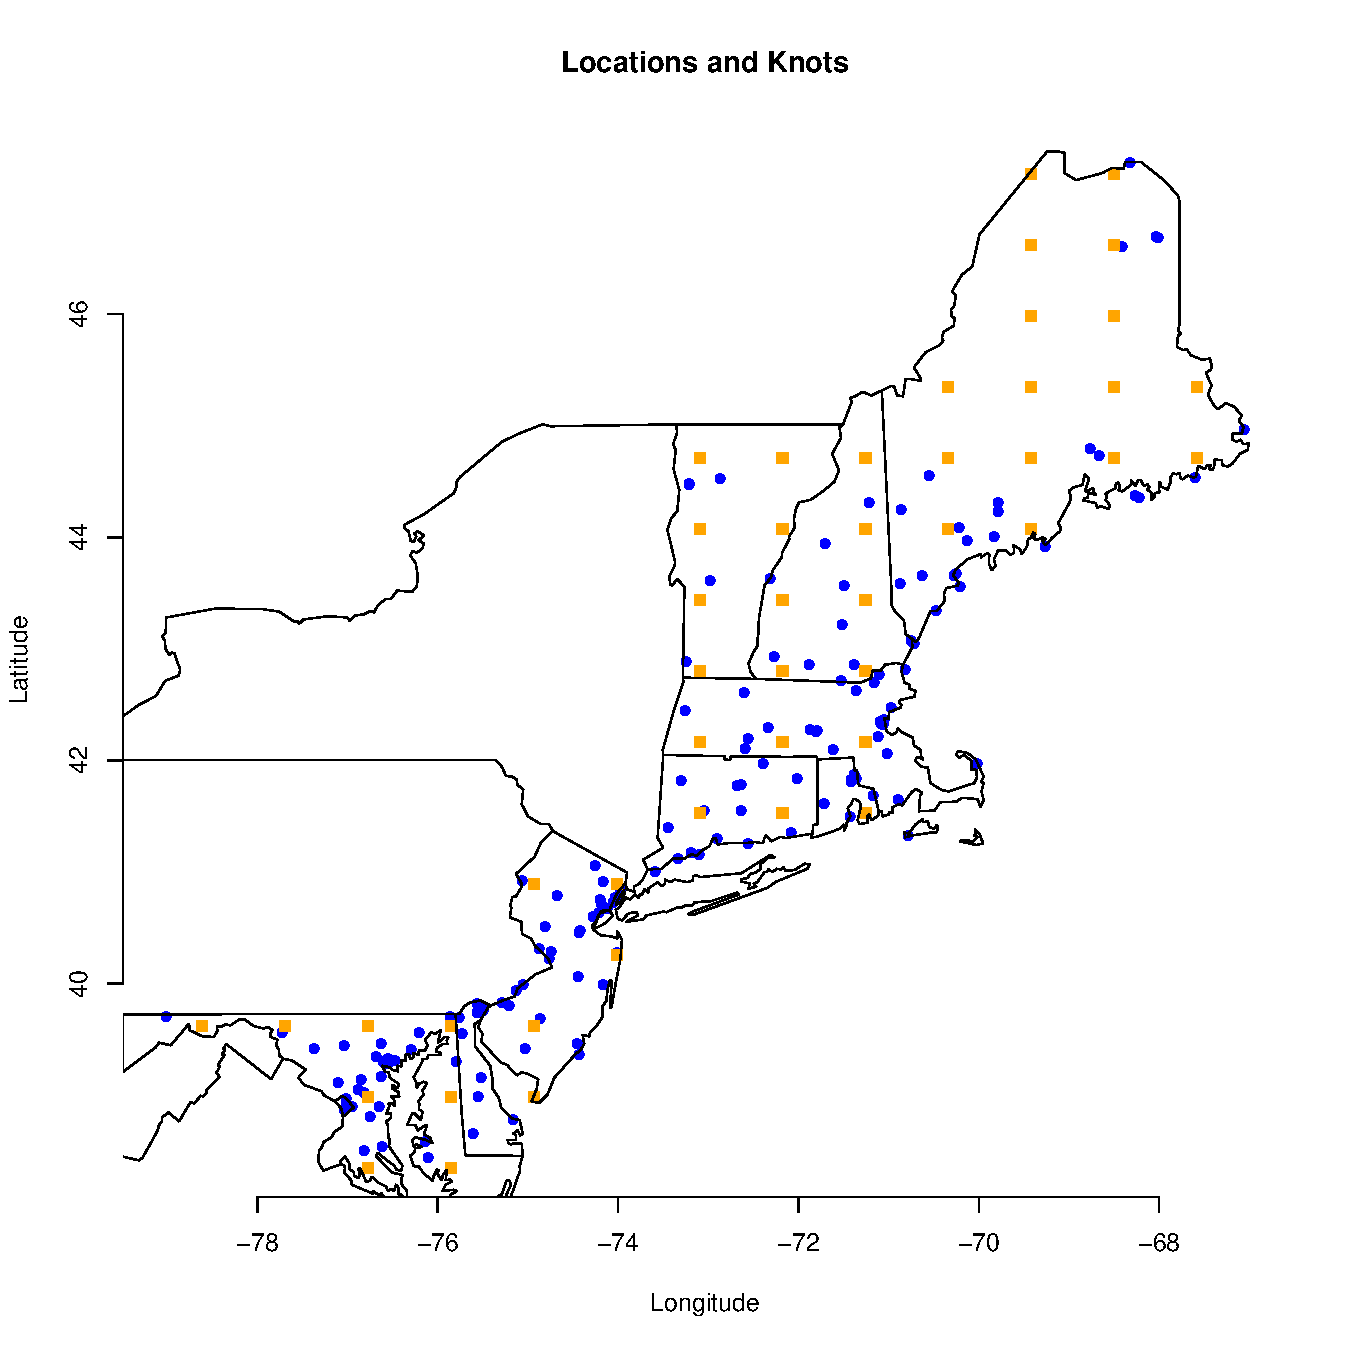
\includegraphics[scale=0.5]{figs/knots.pdf}
\end{center}
\caption{Blue points: all locations where ozone, nitrogen dioxide, and particulate matter were observed. Orange points: the knots used to fit the predictive processes.}
\end{figure}

\subsection*{Trends}

Trends for each variable were considered separately and covariates were selected based off of AIC in linear regression models.
\bigskip

The covariates used for the three variables were:

\begin{table}[ht]
\begin{center}
\begin{tabular}{rl}
Ozone: & northing, northing$^2$, easting $\times$ northing $\times$ altitude \\
NO2:   & northing, altitude, easting $\times$ northing \\
PM2.5: & easting, northing, altitude, northing$^2$ \\
\end{tabular}
\end{center}
\end{table}

\subsection*{Predictive processes}

We first fit univariate predictive processes for the three variables at the specified knots. We then make predictions at the locations where we did not observe one variable (but did observe at least another). For instance, we observed ozone at 104 locations, but nitrogen dioxide at only 37. Of these locations, 20 were common between both ozone and nitrogen dioxide. We would then make predictions for ozone at the remaining $37-20=17$ locations and for nitrogen dioxide at $104-20=84$ locations. We do the same for particulate matter. These predictions became our imputed values, of which there were 158.
 The 158 values were fed into the multivariate modified precitive process.
\bigskip

Surfaces for each variable and for each type of process are shown in Figures 2, 3, and 4. In all three variables, the predictive process is nearly identical to the modified predictive process. There wasn't much of an issue with the univariate processes, except for nitrogen dioxide. For that variable, we observed posterior for samples that looked uniform all along its prior (which was a uniform from $0$ to $100$). Figure 5 shows observed values versus mean predictions (with error bounds) with respect to the modified predictive process.
\bigskip

I had some major issues with the multivariate predictive process that I was unable to figure out. Even after obtaining what looked like somewhat reasonable posterior samples, my predictions were still totally invalid. The surfaces are included to see the deviation (and note, this was after removing several very extreme values and $NaN$s). The observed versus fitted plot for the multivariate fit is omitted since none of it can really be believed anyway.


\begin{figure}[ht]
\begin{center}
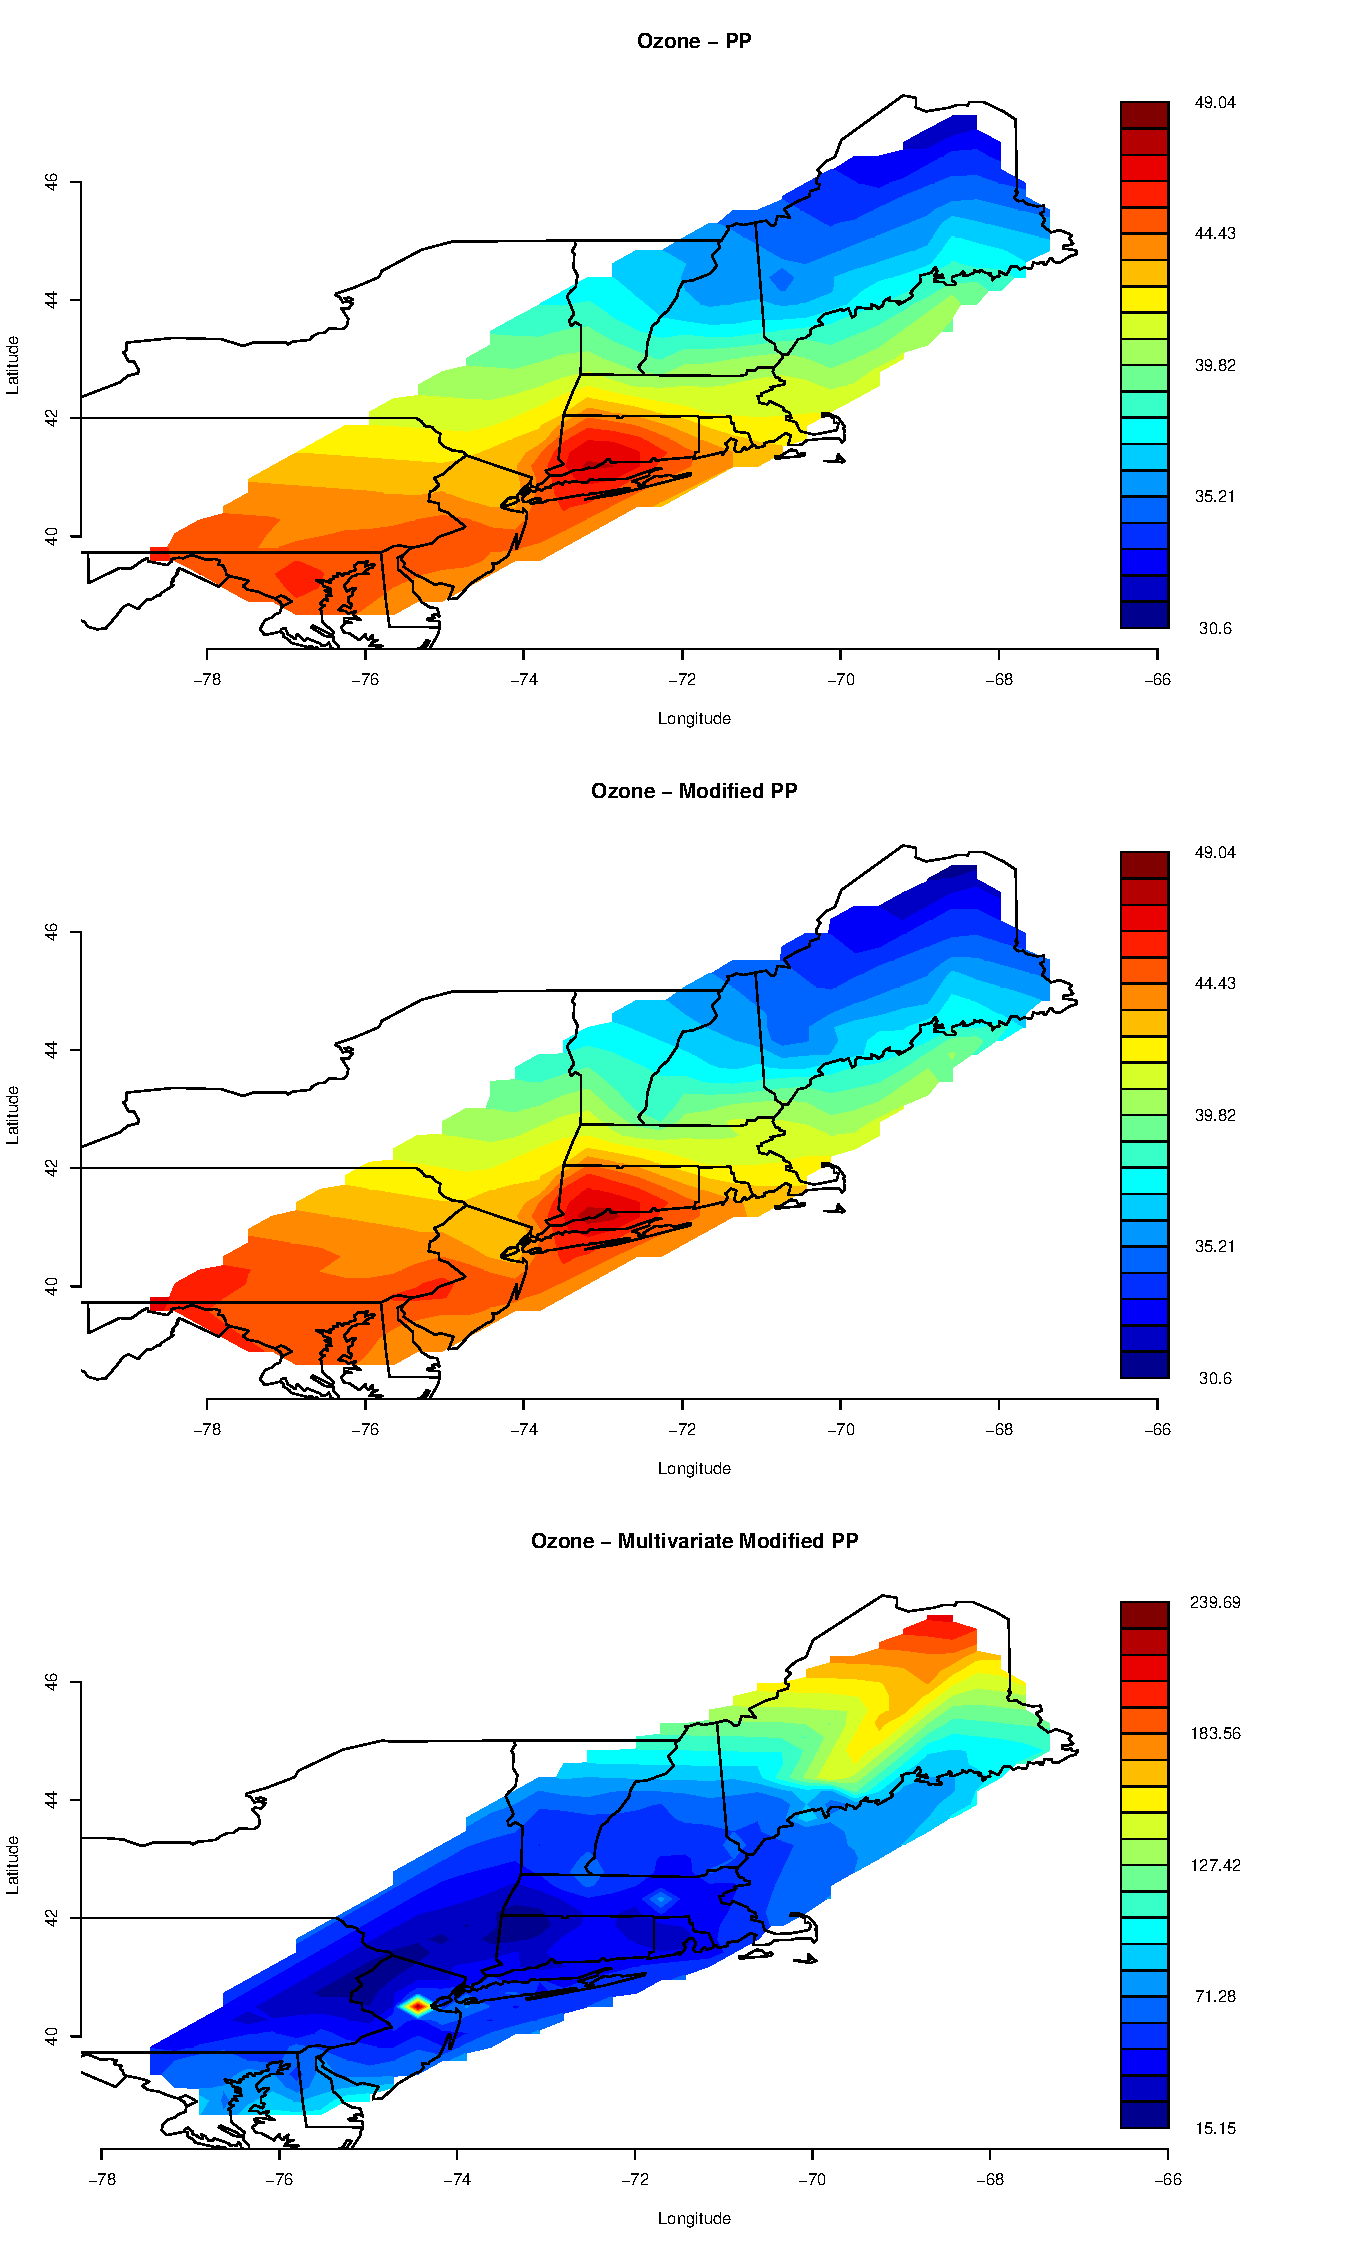
\includegraphics[scale=0.5]{figs/ozone_pp.pdf}
\end{center}
\caption{Ozone predictive processes}
\end{figure}

\begin{figure}[ht]
\begin{center}
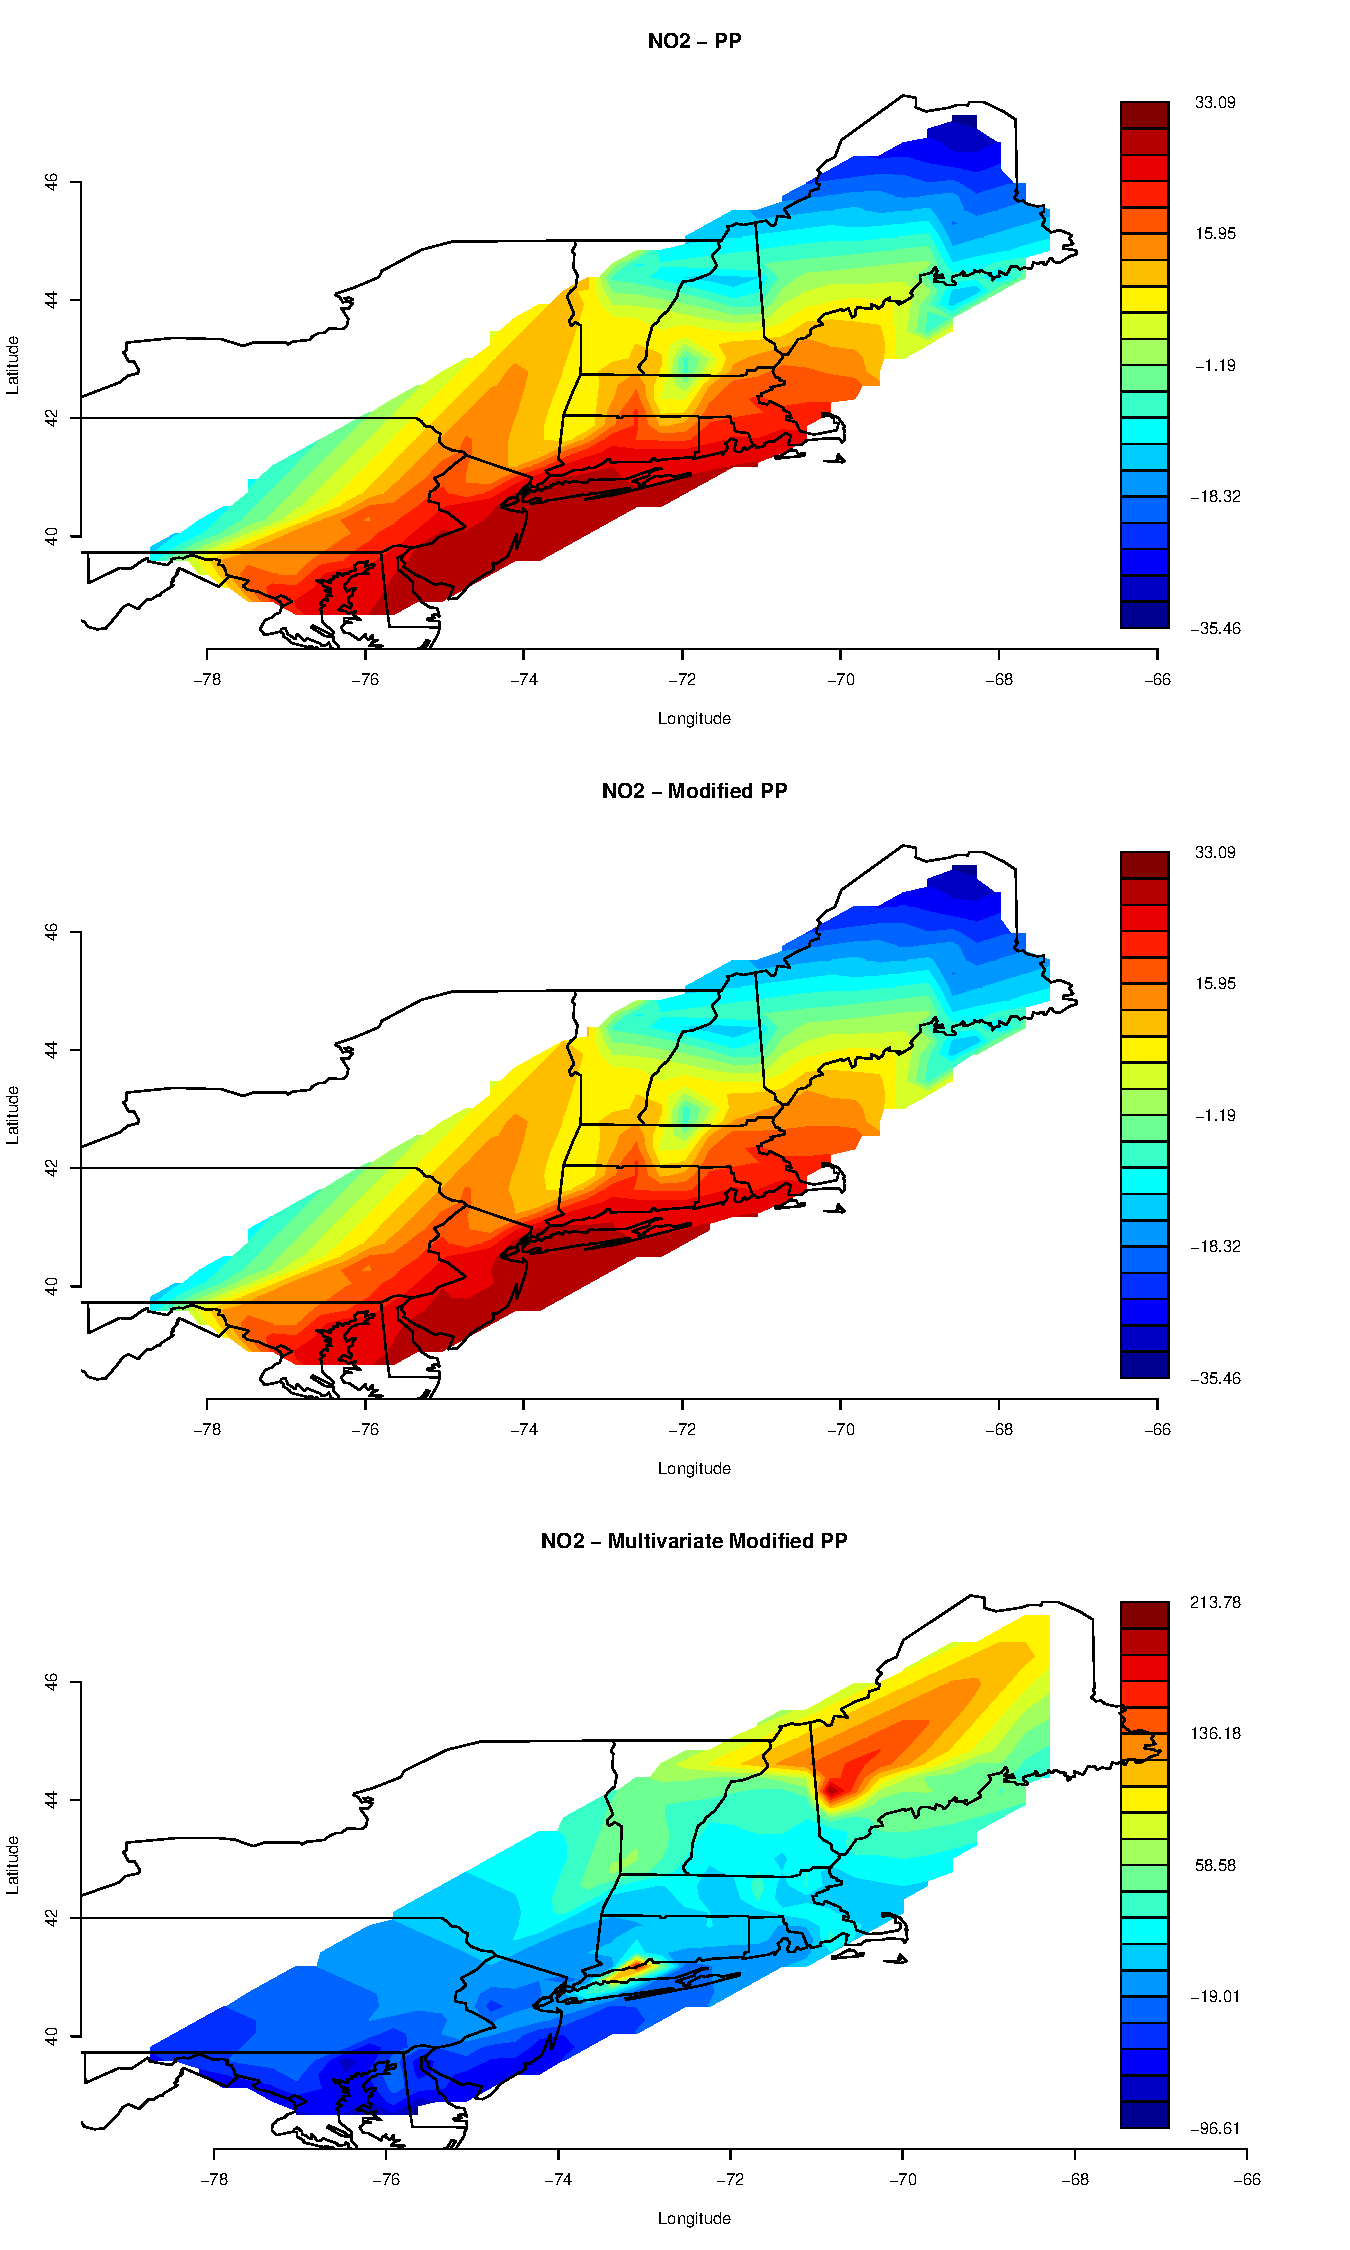
\includegraphics[scale=0.5]{figs/no2_pp.pdf}
\end{center}
\caption{Nitrogen dioxide predictive processes}
\end{figure}

\begin{figure}[ht]
\begin{center}
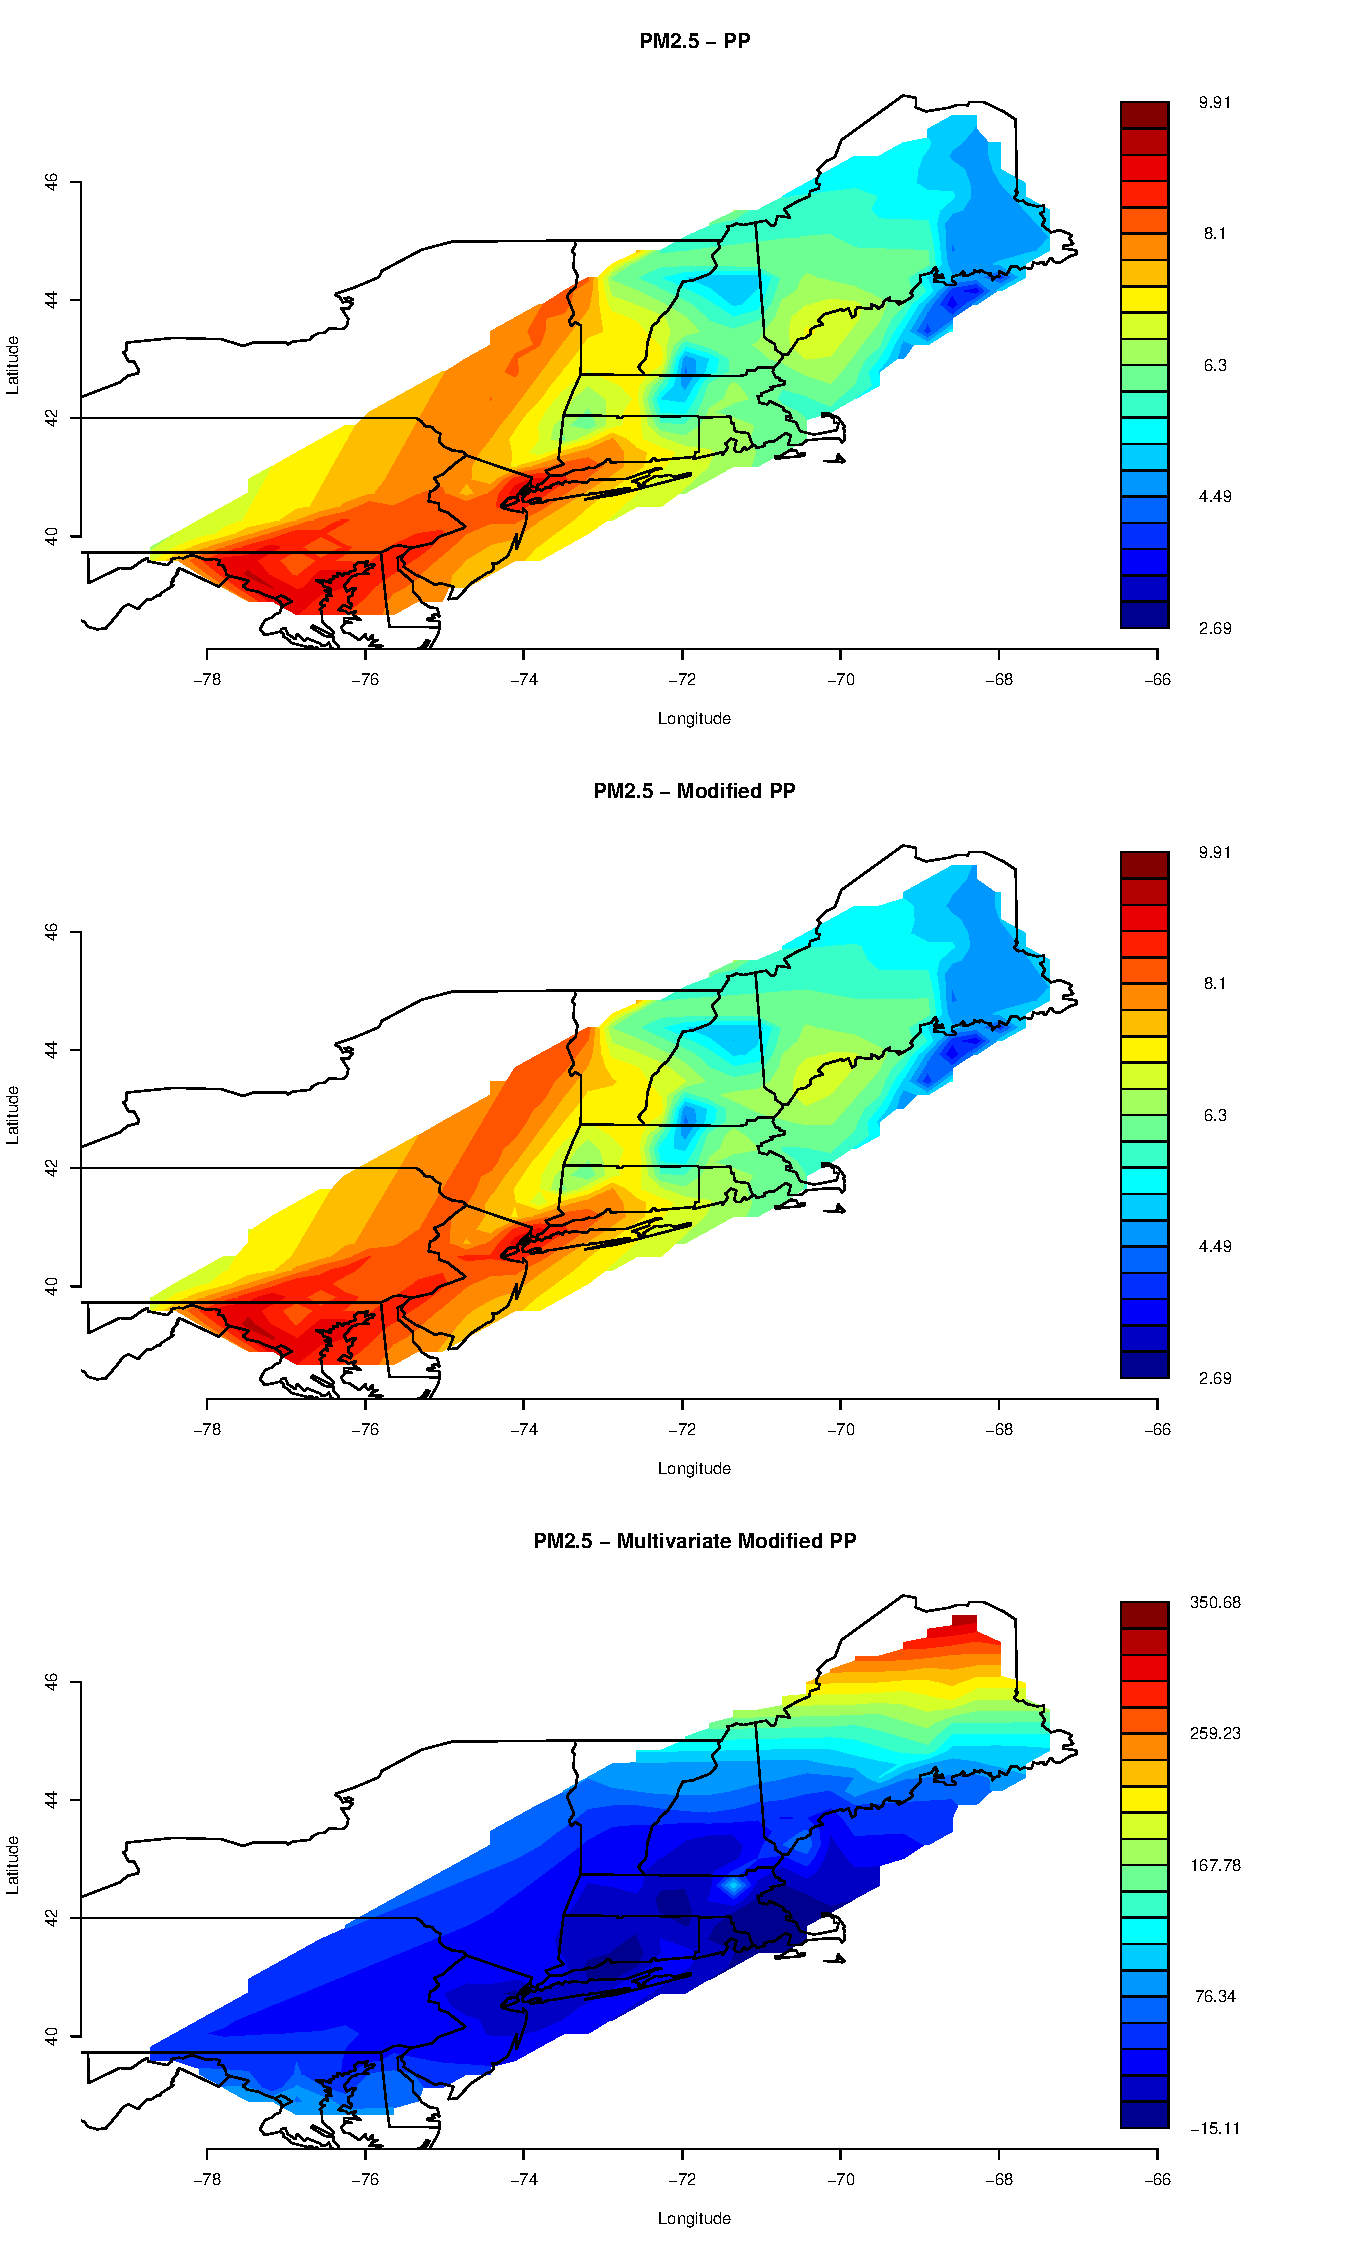
\includegraphics[scale=0.5]{figs/pm25_pp.pdf}
\end{center}
\caption{Particulate matter predictive processes}
\end{figure}

\begin{figure}[ht]
\begin{center}
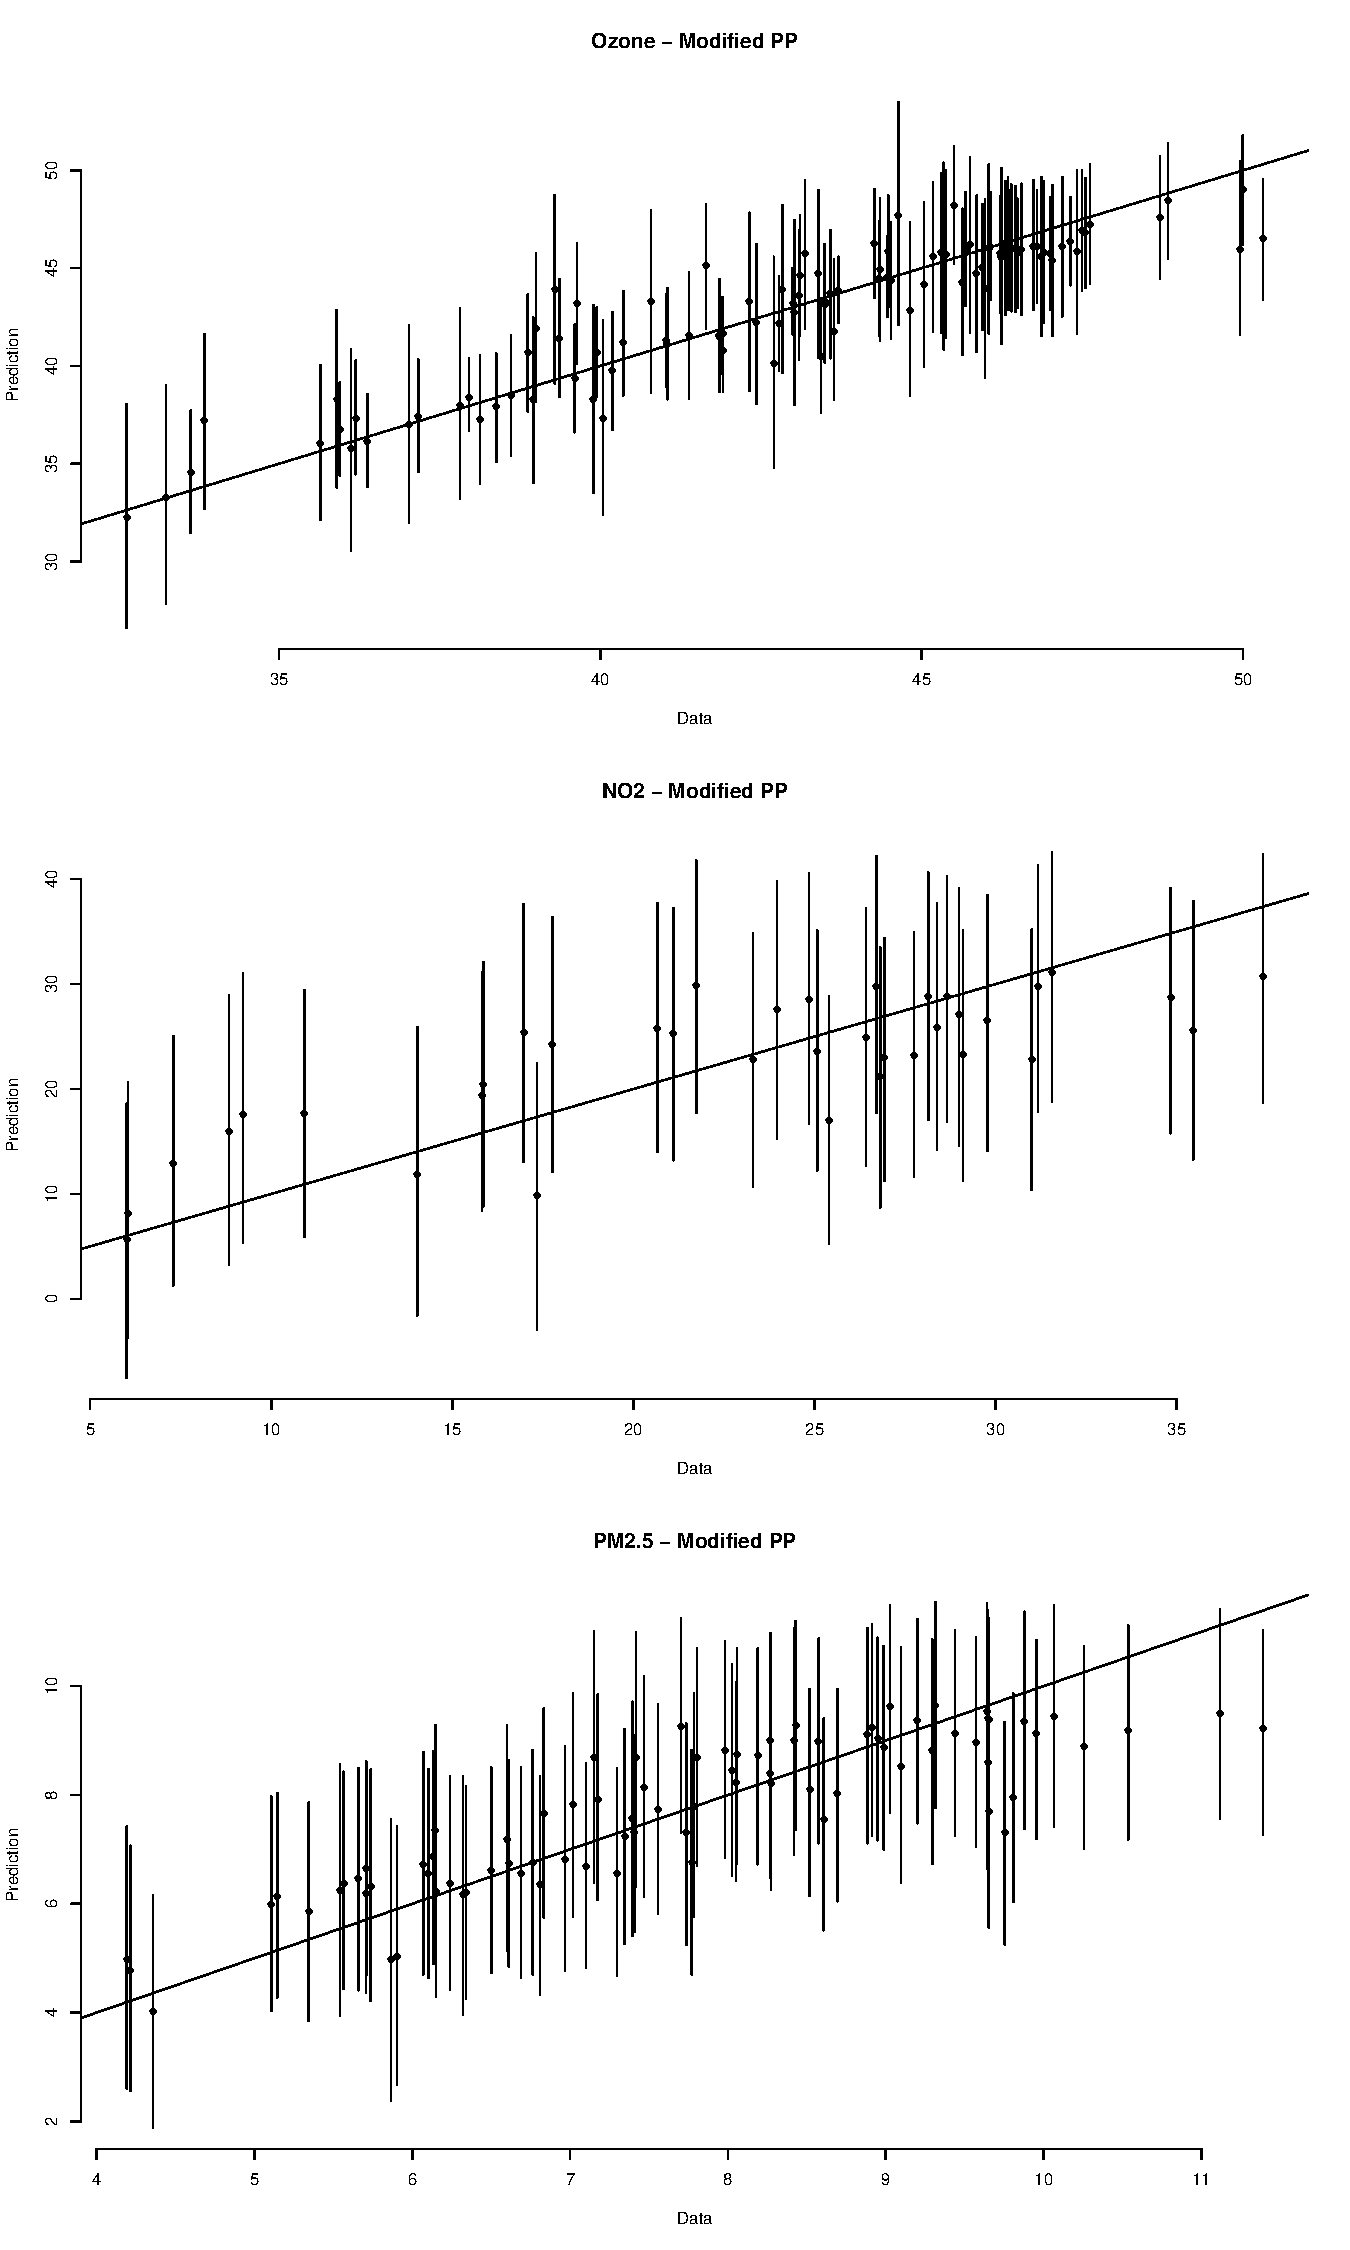
\includegraphics[scale=0.5]{figs/fit.pdf}
\end{center}
\end{figure}





\end{document}
